\section{Experimental Study}
\label{sec:experimental}

\subsection{Data Set}
In introduce what data sets you have used in your experimental study. Real dataset first, then synthetic dataset.

\subsection{Approaches and Measurements}
What approaches tested in the experimental study? Introduce each one with one sentence. Your proposed approaches, the compared existing approaches, random approaches, and so on. 

Why need this paragraph? Readers may have forgotten your solutions, thus just make them recall your solutions through some simple descriptions.

Then introduce the measures you will compare on, such as running time, memory usage, and so on. Usually, control variate method will be used in the experimental study. Define a default setting, then change one parameter in a set of experiments. Make a table to show the configuration, like the example in Table \ref{tab:settings} \cite{cheng2017utility}.

\begin{table}[t]
	\begin{center}
		{\small\scriptsize % \vspace{-1ex}
			\caption{\small Experimental Settings.} \label{tab:settings}
			\begin{tabular}{l|l}
				{\bf \qquad \qquad \quad Parameters} & {\bf \qquad \qquad \qquad Values} \\ \hline \hline
				the number, $m$, of riders  & 1K,  \textbf{3K}, 5K, 8K, 10K\\
				the number, $n$, of vehicles  & 100, \textbf{200}, 300, 400, 500 \\
				the pickup deadline range $[rt^-_{min}, rt^-_{max}]$  & \textbf{[1, 10]}, [10, 30], [30, 60]\\
				the capacity of vehicles $a_j$ & 2, \textbf{3}, 4, 5\\
				the balancing parameters $(\alpha, \beta)$& (0, 0), (1, 0), (0, 1), \textbf{(0.33, 0.33)}\\
				the flexible factor $\varepsilon$ & 1.2, \textbf{1.5}, 1.7, 2\\
				the length $\delta_j$ of time frame $f_j$ & 30 mins\\
				\hline
			\end{tabular}
		}\vspace{-2ex}
	\end{center}
\end{table}

Finally, introduce the running environment of your experimental study. Running on what kind of PCs or servers? Using what programming languages?

\subsection{Experimental Results}

What do you discover or demonstrated in the experimental study? Show the effects of each parameter one by one. Usually, describe results on real dataset first.

Better to have a summary of the interesting points found in the experimental study at the end of this subsection.

\subsection{Adding Figures}
In this subsection, some example of adding figures are introduces. Usually, put figures on the top of pages. Put figures close to their description. 

Below is an example of adding two figures together. Modify the related vspace configuration in head.tex to adjust the global setting. To adjust locally, just add your local spacing command behind them. Parameter ``h'' means ``here''; ``t'' means ``top''; ``!'' means ``mandatory''. In vspace command, I like to use ``ex'', which just a unit and you can use others like ``px''. For other parameters, you can adjust them to see the effects.

\begin{figure}[ht!]\centering \figureTopMargin\vspace{1ex}
	\subfigure[][{\scriptsize Sub Caption1}]{
		\scalebox{0.19}[0.19]{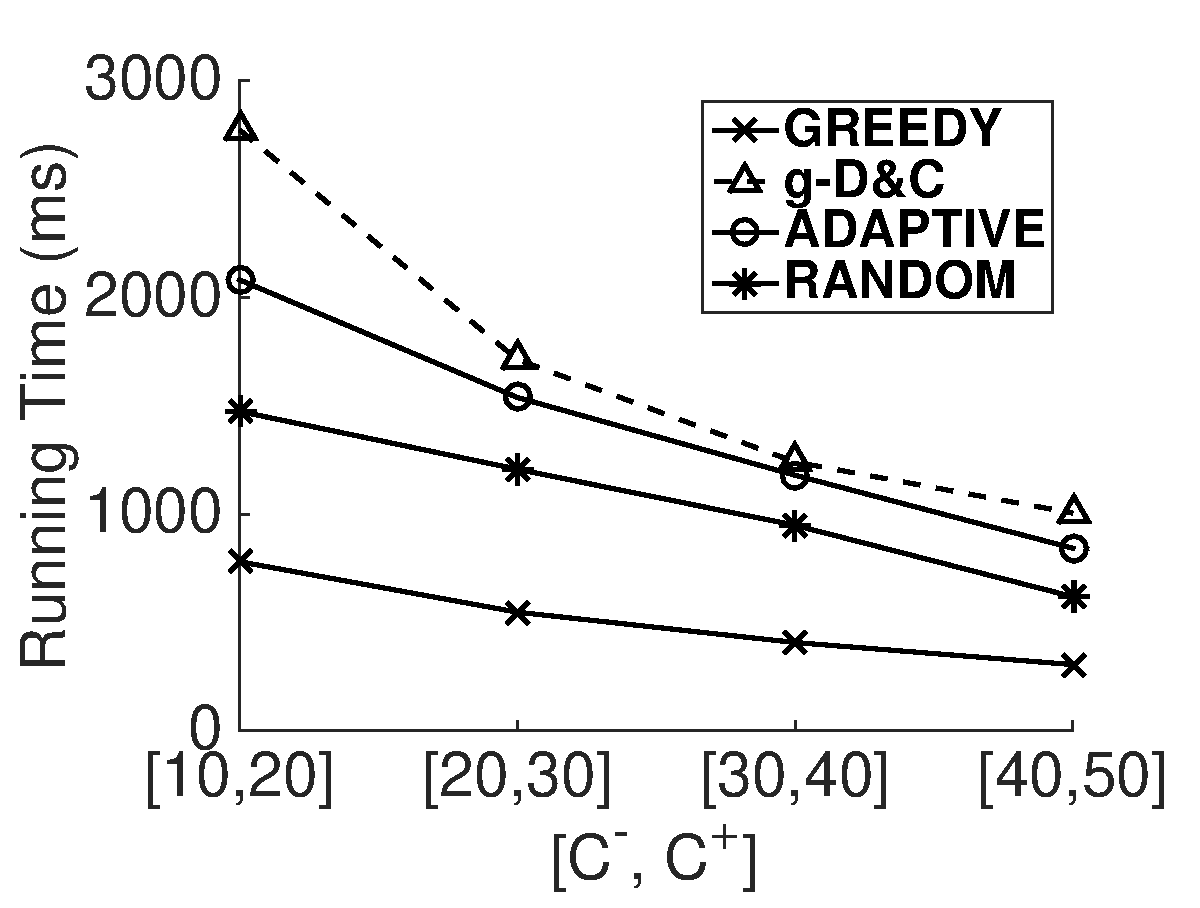
\includegraphics{../figures/example1.eps}}
		\label{subfig:sub_example1}}
	\subfigure[][{\scriptsize Sub Caption2}]{
		\scalebox{0.19}[0.19]{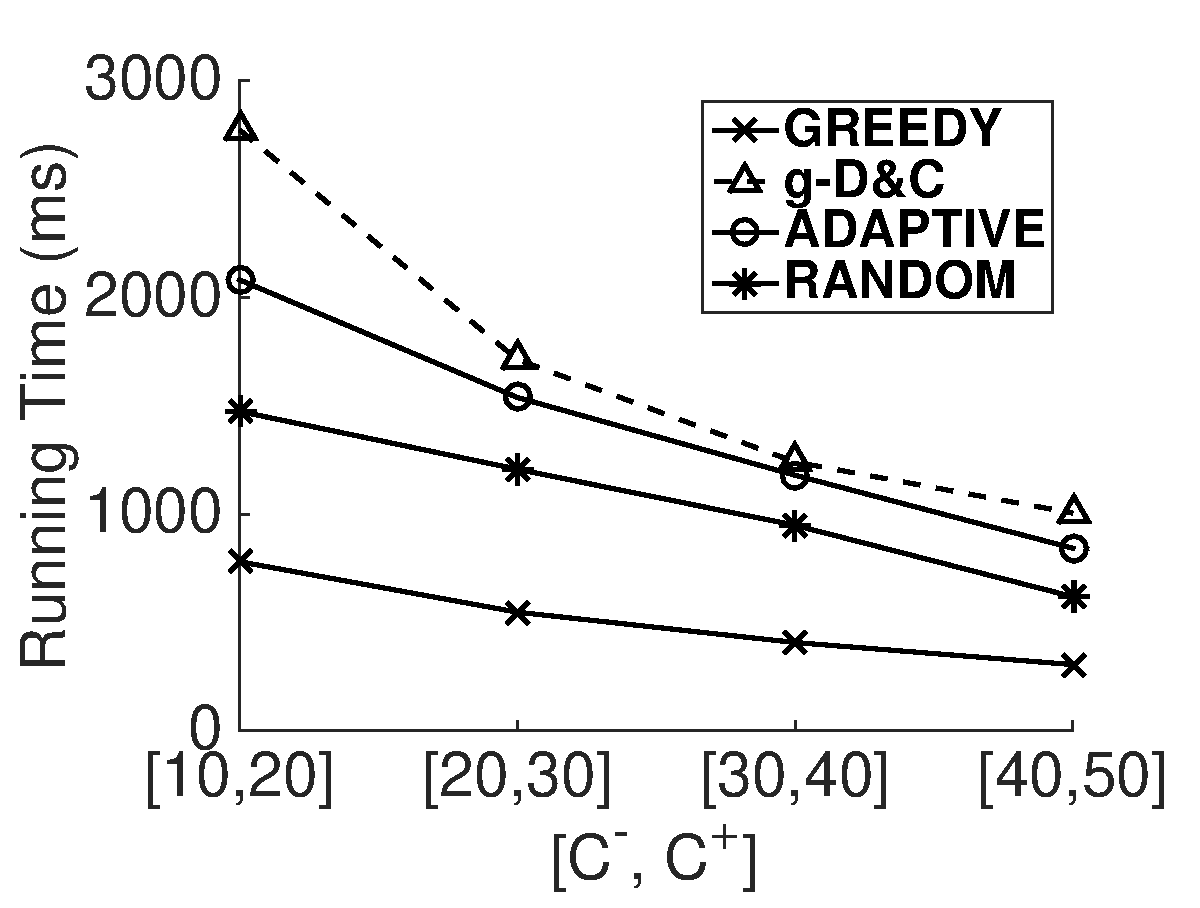
\includegraphics{../figures/example1.eps}}
		\label{subfig:sub_example2}}\figureCaptionMargin
	\caption{\small An Example of Figure.}\figureBelowMargin
	\label{fig:example1}
\end{figure}


Add a bar on top of a group of subfigures, like in Figure \ref{fig:example2}.
\begin{figure}[h!]\centering 
	\subfigure{
		\scalebox{0.4}[0.4]{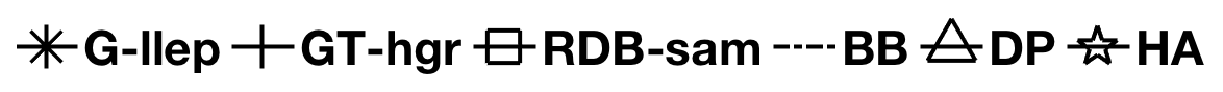
\includegraphics{../figures/bar.eps}}}\hfill\\\vspace{-2ex}
	\addtocounter{subfigure}{-1}
	\subfigure[][{\scriptsize Sub Caption1}]{
		\scalebox{0.19}[0.19]{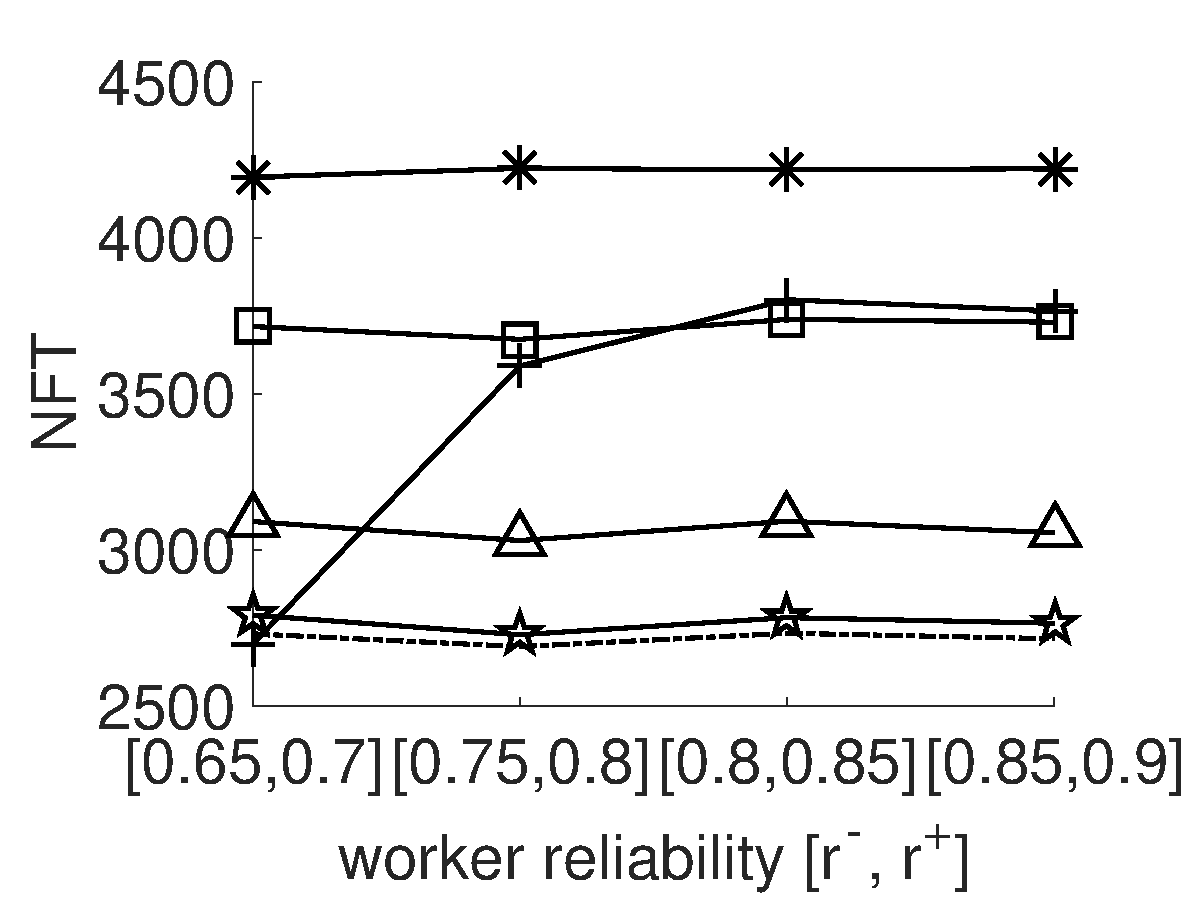
\includegraphics{../figures/example.eps}}
		\label{subfig:sub_example3}}
	\subfigure[][{\scriptsize Sub Caption1}]{
		\scalebox{0.19}[0.19]{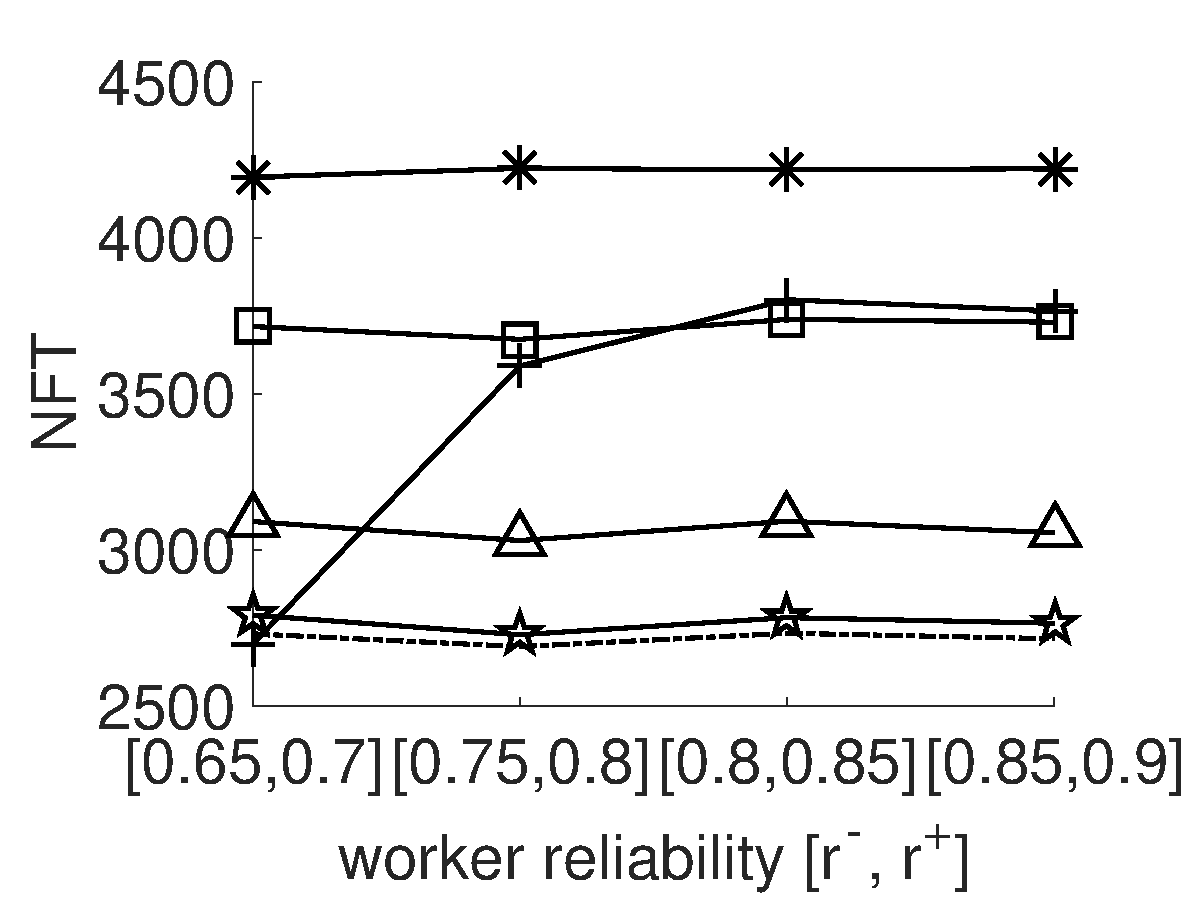
\includegraphics{../figures/example.eps}}
		\label{subfig:sub_example4}}\figureCaptionMargin
	\caption{\small An Example of Figure.}\figureBelowMargin
	\label{fig:example2}
\end{figure}

To draw a figure crossing two columns, like in Figure \ref{fig:example3}.
\begin{figure*}[th!]\centering 
	\subfigure{
		\scalebox{0.4}[0.4]{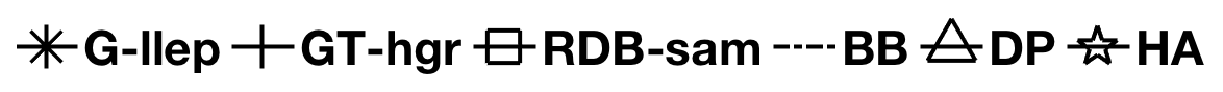
\includegraphics{../figures/bar.eps}}}\hfill\\\vspace{-2ex}
	\addtocounter{subfigure}{-1}
	\subfigure[][{\scriptsize Sub Caption1}]{
		\scalebox{0.18}[0.18]{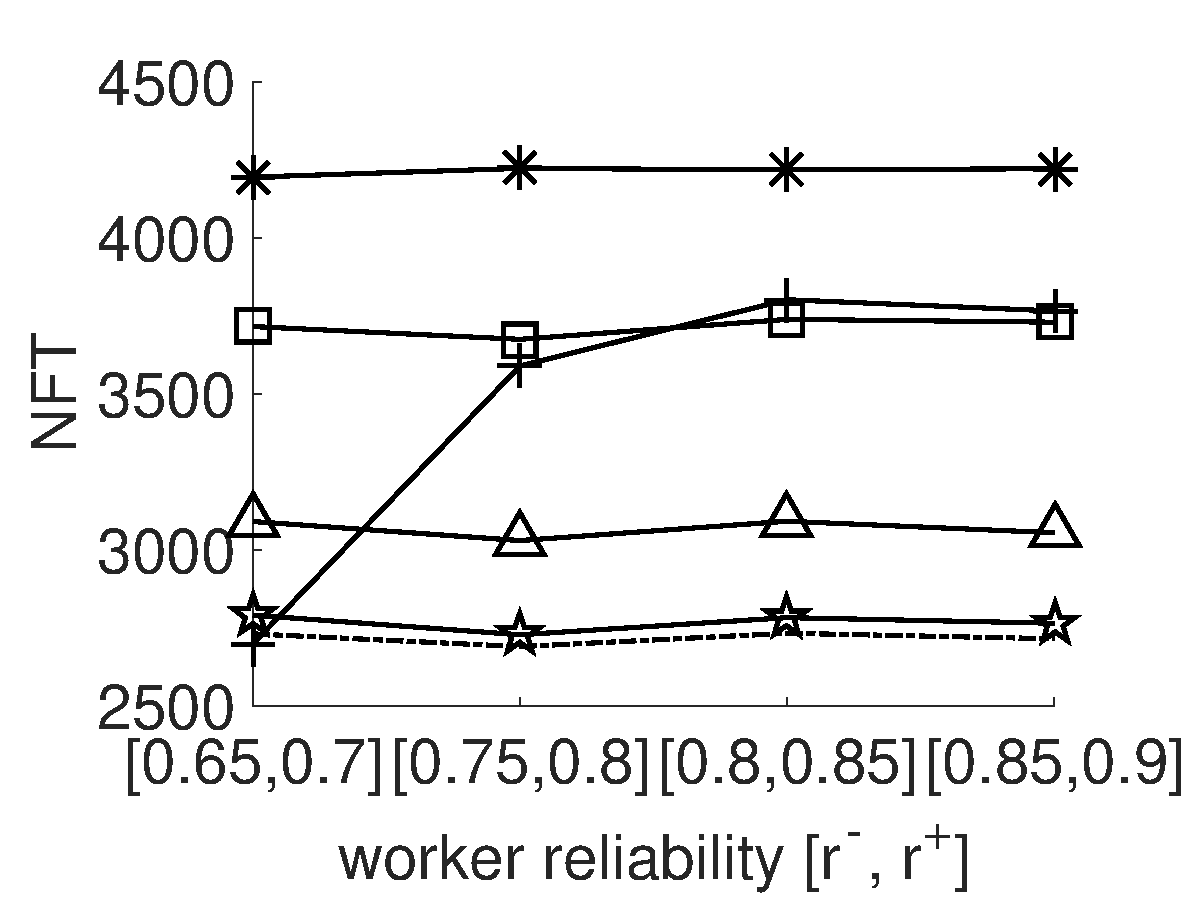
\includegraphics{../figures/example.eps}}
		\label{subfig:sub_example5}}
	\subfigure[][{\scriptsize Sub Caption2}]{
		\scalebox{0.18}[0.18]{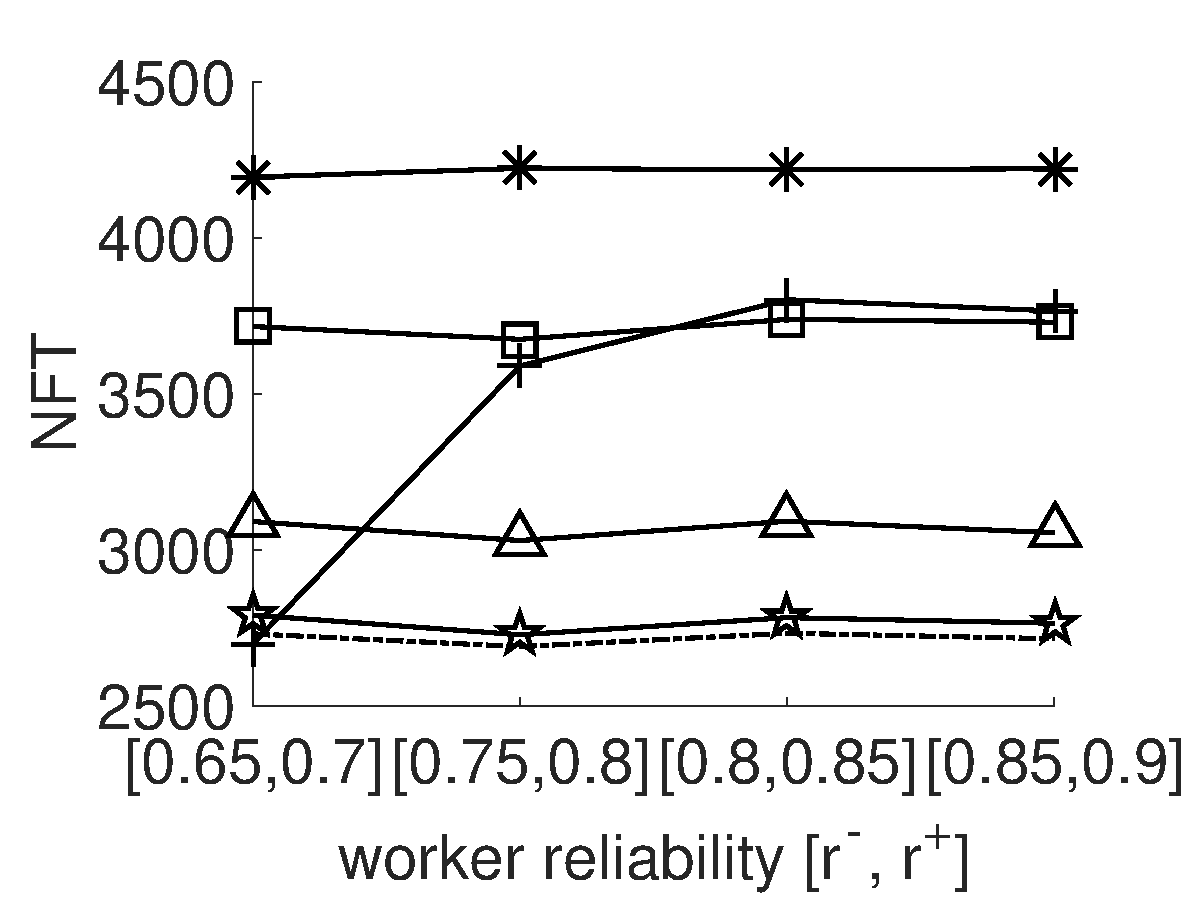
\includegraphics{../figures/example.eps}}
		\label{subfig:sub_example6}}
	\subfigure[][{\scriptsize Sub Caption3}]{
		\scalebox{0.18}[0.18]{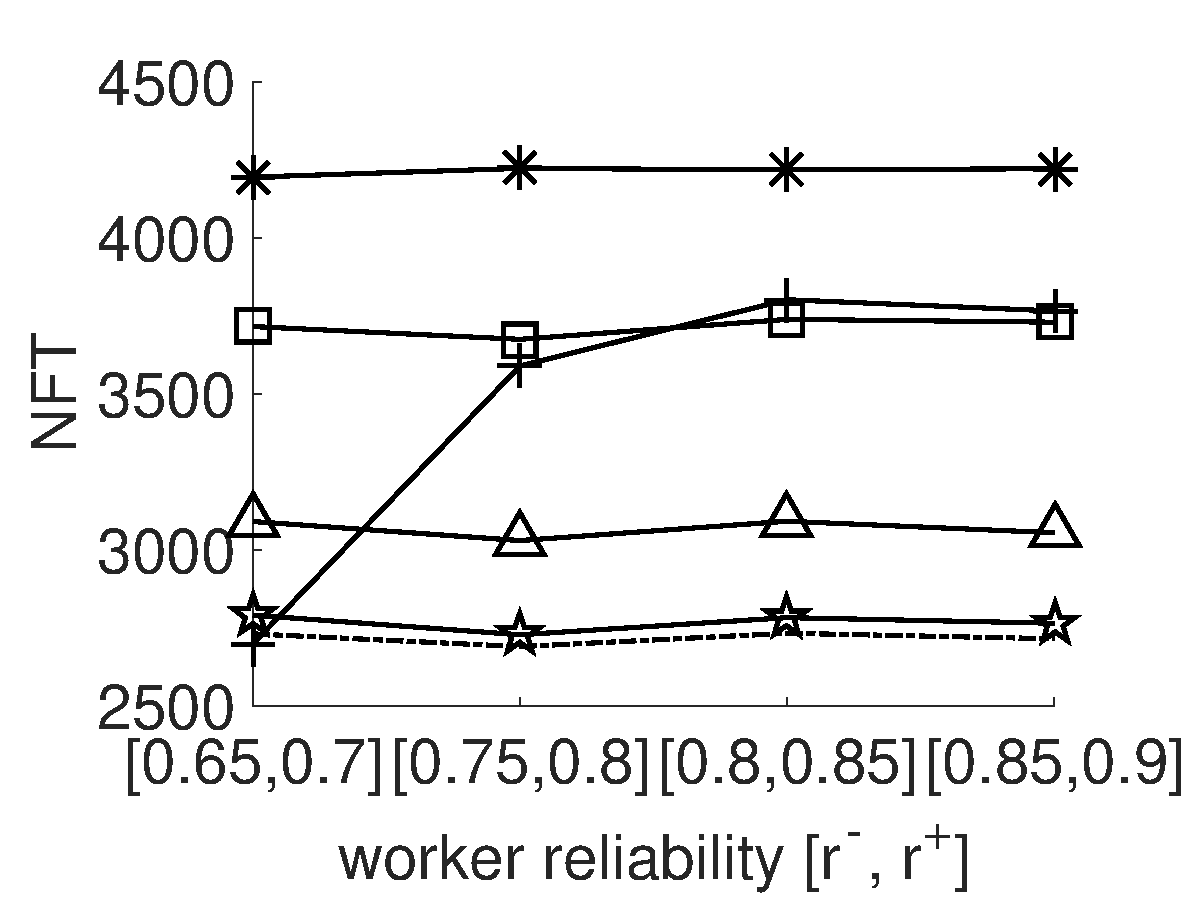
\includegraphics{../figures/example.eps}}
		\label{subfig:sub_example7}}
	\subfigure[][{\scriptsize Sub Caption4}]{
		\scalebox{0.18}[0.18]{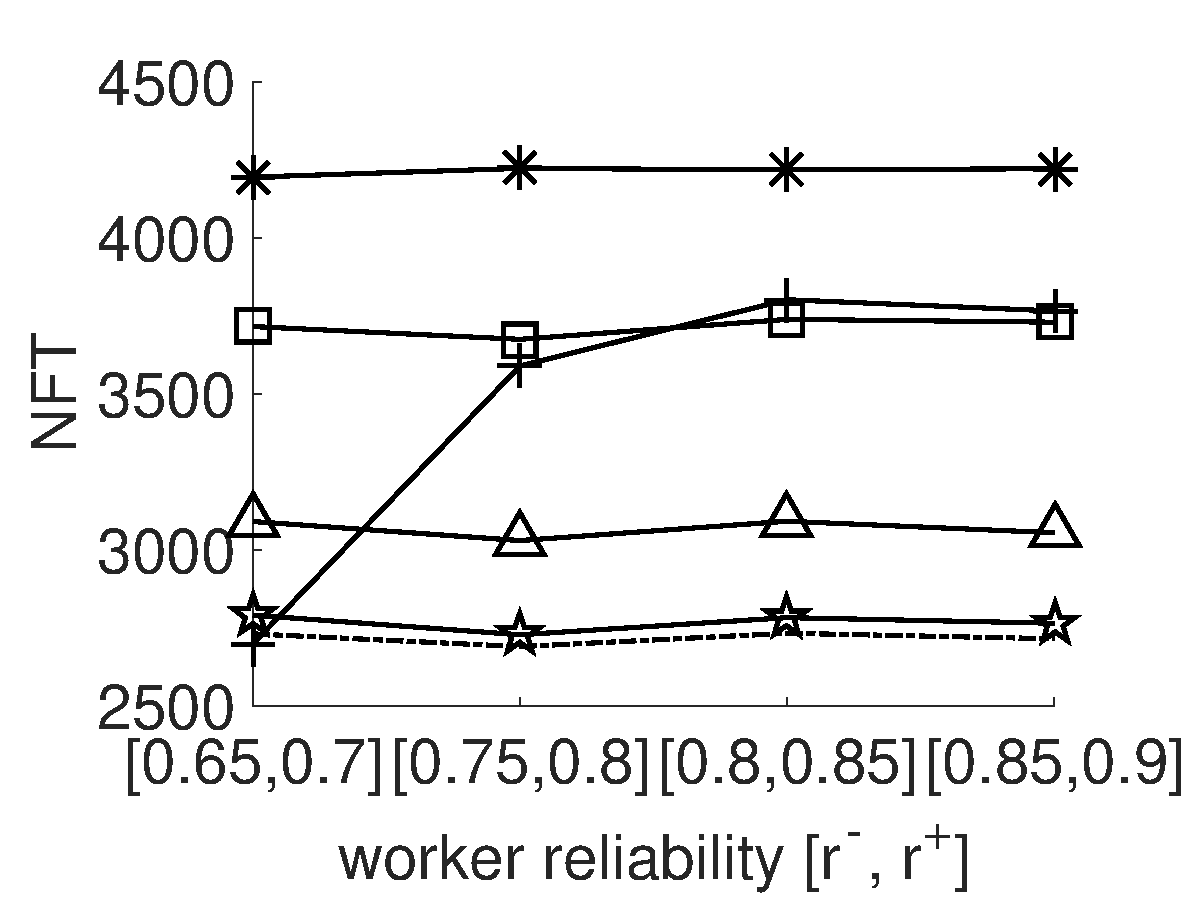
\includegraphics{../figures/example.eps}}
		\label{subfig:sub_example8}}\figureCaptionMargin
	\caption{\small An Example of Figure.}\figureBelowMargin\vspace{-2ex}
	\label{fig:example3}
\end{figure*}

Some suggestions:
\begin{itemize}[leftmargin=*]
	\item Label sub-figures and figures separately. When you describe the particular figure, your can accurately refer to the one you want refer to.
	\item Use eps files! If you need to convert jpg or png to eps, you can try this website: \url{https://www.online-convert.com}, which is the most stable one I can find.
	\item Put figures on the top of pages for better layout. 
	\item Put figures close to their description to ease your readers.
\end{itemize}


Some suggestions/lessons noticed from helping junior PhD students to revise their drafts:
\begin{itemize}[leftmargin=*]
	\item Try to avoid using words like ``naive'', ``obviously'', ``simple'' and so on. 
	\item Don't forget leaving a blank space before (. Bad example: abs(e.g., ddd)
	\item Use aaa~\cite{cheng2016task} in stead of aaa \cite{cheng2016task}, as the first one can avoid strange
    \cite{cheng2016task} new line.
	\item Any Tables, Figures, Algorithms or other similar components in your draft should be discussed with some natural language. Don't simply put them in your draft as no one know their purposes unless you describe them clearly. 
	\item Numbered equations should be referred somewhere in your draft. If not, just don't number them. You can add ``$\backslash$notag'' behind an equation to suppress its numbering.
\end{itemize}